\section{Signal Processing and Conditioning}
\title{Signal Processing and Conditioning}  

\begin{frame}[plain]
    \titlepage
\end{frame}

%%%%%%%%%%%%%%%%%%%%%%%%%%%%%%%%%%%%%%%%%%%%%%%%%%%%%%%%%%%%%
%% Introduction to the p-n junctions %%
%%%%%%%%%%%%%%%%%%%%%%%%%%%%%%%%%%%%%%%%%%%%%%%%%%%%%%%%%%%%%

\begin{frame}{Measurement and Signal Processing}
\small
\textbf{Goal:} Transform a physical phenomenon into a measurable and interpretable electrical signal.

\begin{itemize}
    \item Measurement = objective assignment of numerical value to a property.
    \item Signal processing ensures that sensor outputs are usable by controllers or digital systems.
    \item Conditioning bridges the physical world and the information world.
\end{itemize}

\begin{block}{Core Idea}
Sensors $\Rightarrow$ Signal Conditioning $\Rightarrow$ Data Conversion $\Rightarrow$ Processing $\Rightarrow$ Display/Control
\end{block}
\end{frame}


\begin{frame}{Elements of a Measurement System}
\centering
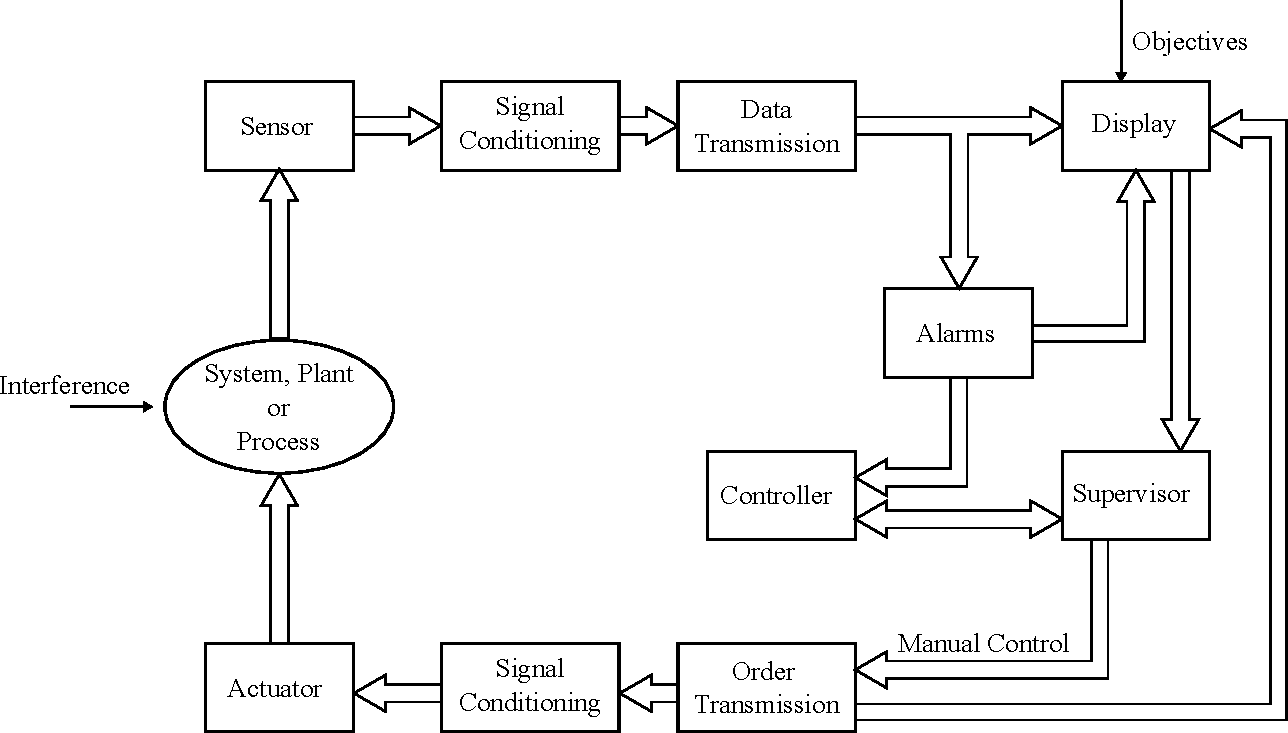
\includegraphics[scale=0.6]{fig/lec03/measurement_loop.pdf}

\end{frame}


\begin{frame}{Elements of a Measurement System}
\textbf{Subsystems:}
\begin{columns}
\column{0.5\textwidth}
\begin{enumerate}
    \item \textbf{Sensor / Transducer} - converts physical to electrical signals.
    \item \textbf{Signal Conditioning} - amplifies, filters, linearizes.
    \item \textbf{Data Transmission} - carries signals to control or display unit.
    \item \textbf{Controller / Processor} - interprets and acts upon data.
    \item \textbf{Actuator} - applies control action to the system or process.
\end{enumerate}
\column{0.5\textwidth}
\centering
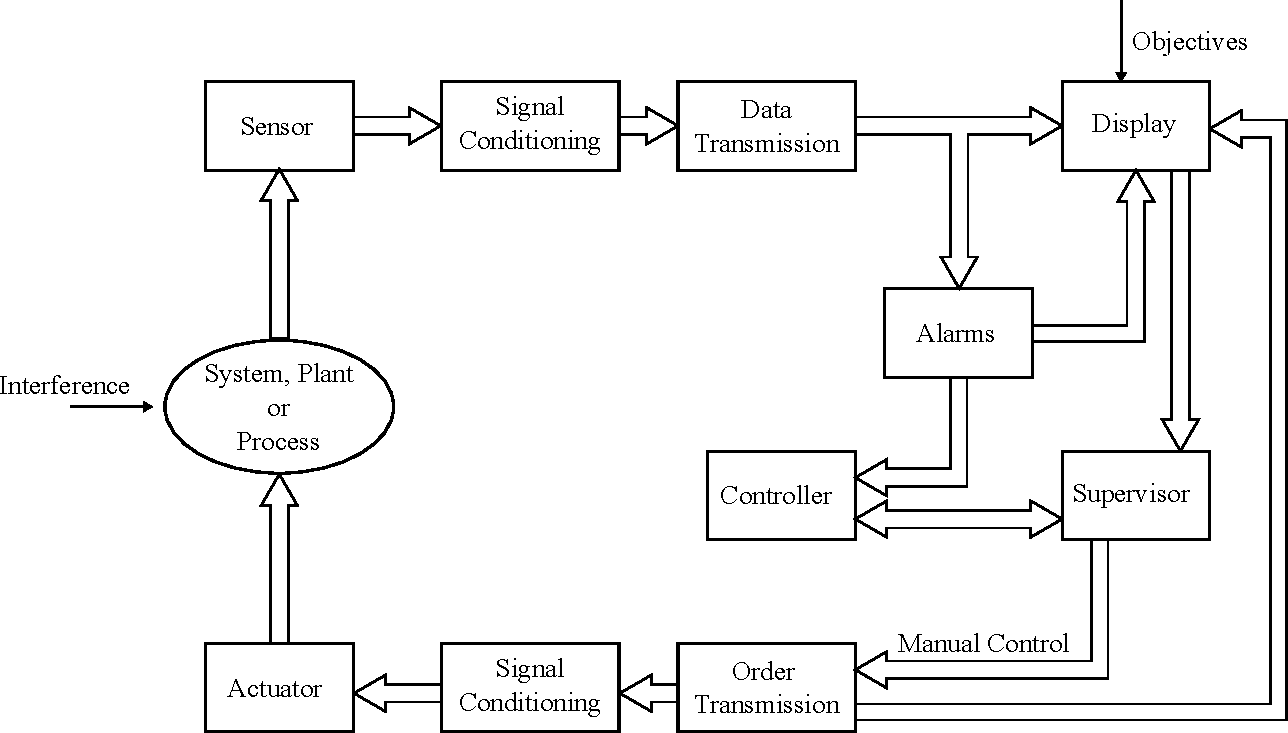
\includegraphics[scale=0.35]{fig/lec03/measurement_loop.pdf}
\end{columns}

\end{frame}

\begin{frame}{Transducers, Sensors, and Actuators}
\small
\textbf{Transducer:} Converts energy from one form to another. \\ 
\textbf{Sensor:} Input transducer--detects a physical variable and converts it to an electrical signal.  \\
\textbf{Actuator:} Output transducer--converts electrical signals into mechanical motion or other actions.

\begin{block}{Key Concepts}
\begin{itemize}
    \item Always some energy flow from measured system to sensor $\Rightarrow$ avoid loading effect.
    \item Six domains: mechanical, thermal, magnetic, electrical, chemical, radiation.
    \item Sensors with electric outputs dominate modern systems.
\end{itemize}
\end{block}
\end{frame}

\begin{frame}{Advantages of Electrical Measurement Systems}
\small
\begin{enumerate}
    \item Electric parameters vary with almost any physical quantity (temperature, strain, pressure).
    \item Signal energy can be amplified  -- minimal disturbance to measured system.
    \item Wide availability of integrated circuits for conditioning and processing.
    \item Data can be easily recorded, transmitted, and displayed electronically.
    \item Electrical signals are versatile and compatible with digital systems.
\end{enumerate}
\textbf{Primary sensor:} interacts with the measurand (e.g., diaphragm senses pressure).  \\ 
\textbf{Secondary sensor:} converts the effect into an electrical signal (e.g., strain gauge).

\begin{itemize}
    \item Example: Pressure $\rightarrow$ diaphragm deformation $\rightarrow$ resistance change $\rightarrow$ voltage signal.
    \item Full sensor assembly includes sensing element + package + leads.
    \item The raw signal typically has low amplitude and needs conditioning.
\end{itemize}
\end{frame}


\begin{frame}{Signal Conditioning}
\begin{columns}
\column{0.5\textwidth}
\textbf{Signal conditioning:} prepares sensor output for transmission, digitization, or display.

\begin{itemize}
    \item Functions: amplification, filtering, impedance matching, level shifting, modulation/demodulation.
    \item Converts weak analog signals (mV range) to standard ranges ($\pm 10$ V or 4–20 mA).
    \item Analog-to-digital converters (ADCs) need well-conditioned inputs.
    \item Final display may be analog (pointer, gauge) or digital (numeric, bar graph).
\end{itemize}
\column{0.5\textwidth}
\centering
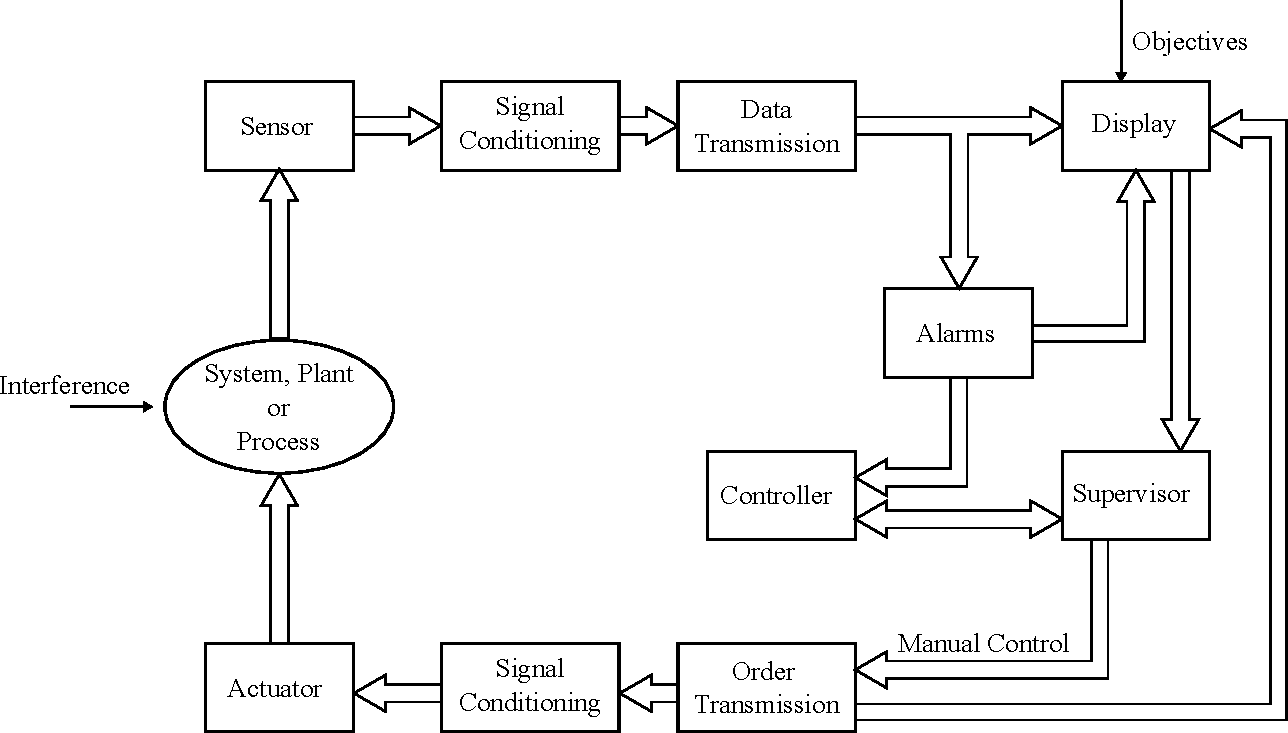
\includegraphics[scale=0.35]{fig/lec03/measurement_loop.pdf}
%\caption*{Signal conditioning stage highlighted in the measurement chain.}
\end{columns}

\end{frame}


\begin{frame}{Interfaces and Data Domains}
\small
\textbf{Measurement systems involve multiple data domains:}
\begin{itemize}
    \item Domains describe how information is represented or transmitted.
    \item Interface stages (ADC, DAC) convert between domains.
\end{itemize}

\textbf{Common domains:}
\begin{itemize}
    \item \textbf{Analog:} signal amplitude represents information (voltage, current).
    \item \textbf{Time:} information encoded in timing (frequency, phase, pulse width).
    \item \textbf{Digital:} information represented numerically (binary codes, counts).
    \item \textbf{Chemical/Physical:} domains prior to conversion to electrical form.
\end{itemize}
\end{frame}

\begin{frame}{Data Domain Representation}
\begin{columns}
\column{0.35\textwidth}
\textbf{Information carriers:}
\begin{itemize}
    \item \textbf{Analog domain:} amplitude (voltage/current).
    \item \textbf{Time domain:} period, frequency, or phase.
    \item \textbf{Digital domain:} pulse count, word code.
\end{itemize}
\textit{Each stage in the measurement chain may operate in a different domain, requiring proper interfacing and conversion.}
\column{0.65\textwidth}
\centering
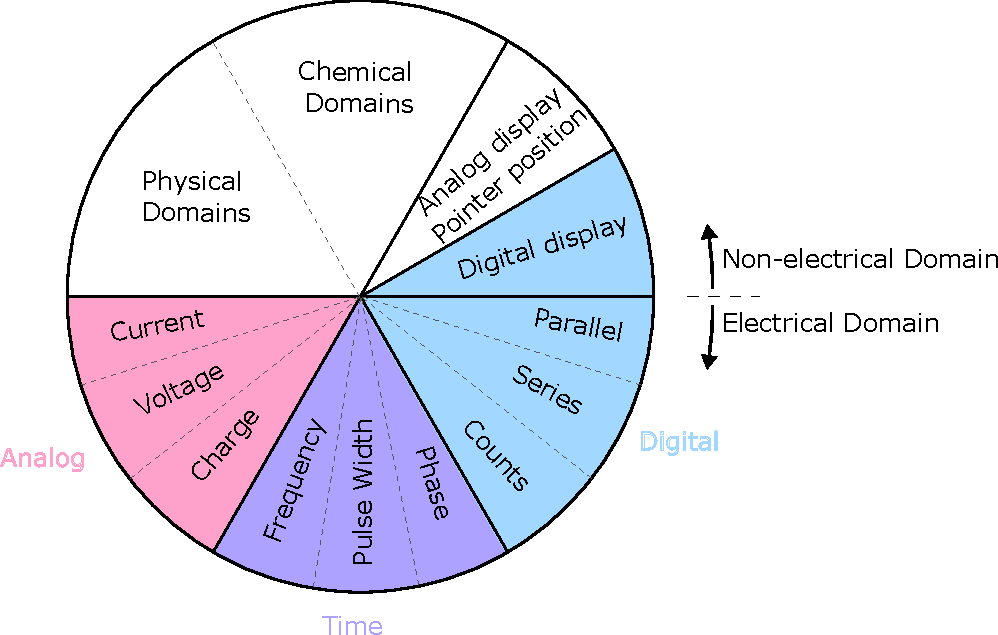
\includegraphics[scale=0.65]{fig/lec03/data_domains.pdf}
\end{columns}
\end{frame}


\begin{frame}{Direct Adjustment Indirect Measurements}
\small
\textbf{Direct measurement:}
\begin{itemize}
    \item Comparison with a reference standard (e.g., weighing scale, voltmeter).
\end{itemize}

\textbf{Indirect measurement:}
\begin{itemize}
    \item Computed from other quantities using physical laws.
    \item Examples:
    \begin{itemize}
        \item Power = Voltage × Current
        \item Distance = $\int$ speed dt
    \end{itemize}
\end{itemize}
\vspace{4pt}
\textbf{Most modern measurements are indirect and require signal processing.}
\end{frame}


\begin{frame}{Summary and Context for Next Topics}
\small
\textbf{You have learned:}
\begin{itemize}
    \item The structure of a measurement and control system.
    \item Roles of transducers, sensors, actuators, and conditioners.
    \item The flow of information through different domains.
\end{itemize}

\textbf{Next lectures:}
\begin{itemize}
    \item Resistive and bridge circuits for signal generation.
    \item Operational amplifiers in conditioning.
    \item ADCs, DACs, sampling, and quantization.
\end{itemize}

\end{frame}



\begin{frame}{Overview of Signal Processing and Calibration}
\small
\textbf{Goal:} Convert a physical quantity/phenomenon into a usable electrical/digital signal decision

\begin{itemize}
  \item Sensors generate low-level, often non-linear, analog outputs.
  \item Signal processing and conditioning amplify, filter, linearize, and standardize them.
  \item Calibration ensures accuracy and removes offset, drift, and disturbances.
\end{itemize}

\textbf{Key challenges:}
\begin{enumerate}
  \item Very small signal levels $\rightarrow$ require amplification.
  \item Influence of disturbance variables (e.g. temperature).
  \item Nonlinear characteristic curves $\rightarrow$ need linearization and filtering.
\end{enumerate}
\textbf{Output types:}
\begin{itemize}
  \item Binary (on/off)
  \item Pulse / frequency encoded
  \item Analog continuous signals
\end{itemize}
\end{frame}

\begin{frame}{Signal Conditioning Functions}
\begin{itemize}
    \item \textbf{Amplification:} Boosts weak sensor signals to usable levels.
    \item \textbf{Filtering:} Removes noise and unwanted frequency components.
    \item \textbf{Linearization:} Corrects nonlinear sensor outputs.
    \item \textbf{Impedance Matching:} Ensures proper signal transfer between stages.
    \item \textbf{Level Shifting:} Adjusts signal baseline for compatibility.
    \item \textbf{Modulation/Demodulation:} Prepares signals for transmission or extraction.
    \item \textbf{Isolation:} Prevents ground loops and protects against high voltages.
    \item \textbf{Calibration:} Adjusts system to ensure accurate measurements.
    \item \textbf{Conversion:} Transforms signals between analog and digital domains.
    \item \textbf{Data Transmission:} Sends signals over distances without degradation.
\end{itemize}
\end{frame}

\begin{frame}{Common Signal Conditioning Techniques}
\begin{itemize}
    \item \textbf{Bridge Circuits:} Convert resistance changes (e.g., strain gauges) into voltage signals.
    \item \textbf{Operational Amplifiers:} Used for amplification, filtering, and buffering.
    \item \textbf{Filters:} Low-pass, high-pass, band-pass, and notch filters to manage frequency content.
    \item \textbf{Analog-to-Digital Converters (ADCs):} Convert analog signals to digital form for processing.
    \item \textbf{Digital-to-Analog Converters (DACs):} Convert digital signals back to analog form.
    \item \textbf{Multiplexers:} Allow multiple sensor signals to be processed by a single conditioning circuit.
    \item \textbf{Isolation Amplifiers:} Provide galvanic isolation between input and output.
    \item \textbf{Temperature Compensation Circuits:} Mitigate effects of temperature variations on sensor outputs.
    \item \textbf{Signal Modulators/Demodulators:} Prepare signals for transmission over long distances.
    \item \textbf{Data Transmission Protocols:} Ensure reliable communication between sensors and processing units.
\end{itemize}
\end{frame}

\begin{frame}{Introduction to D.C. and A.C. Bridges}
\small
\textbf{Objective:} Bridge circuits are used to measure unknown resistance, capacitance, or inductance precisely by comparing with known components.

Conversion of tiny sensor variations (strain gauge, RTD, capacitive sensor) into measurable voltages and principles of null deflection help to curtain noise and improve accuracy.

\begin{itemize}
    \item Based on the principle of \textbf{null deflection} — when the bridge is balanced, no current flows through the detector.
    \item Used extensively for \textbf{signal conditioning} in sensors and transducers.
    \item D.C. bridges → resistive transducers (strain gauges, resistance temperature detectors (RTDs)).\\
          A.C. bridges → reactive transducers (inductive, capacitive).
\end{itemize}

\begin{block}{Bridge Balance Principle}
\[
\frac{Z_1}{Z_2} = \frac{Z_3}{Z_4}
\]
At balance: $V_X = V_Y$ and detector current = 0.
\end{block}
\end{frame}


\begin{frame}{Introductory Example: Half-Bridge Measurement}
\small
\textbf{Half-bridge concept:}
\[
e_o = e_i \frac{R_2}{R_1 + R_2}, \qquad [e_o, e_i\ \text{in V}]
\]
where:
\[
R_1 = R + \Delta R, \quad R_2 = R.
\]
\begin{columns}
\column{0.65\textwidth}
\textbf{Issues:}
\begin{itemize}
    \item Always produces non-zero offset: $e_o(e_{\text{stimulus}=0}) \neq 0$.
    \item Temperature drift affects balance.
\end{itemize}

\textbf{Use cases:}
\begin{itemize}
    \item Basic resistance sensing demonstration.
    \item Precursor to full Wheatstone bridge.
\end{itemize}
\column{0.35\textwidth}
\begin{figure}
  \vspace{-2cm}
    \centering
    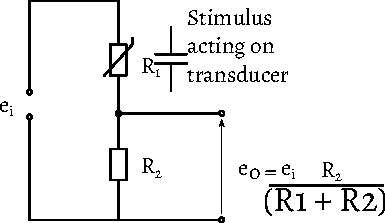
\includegraphics[scale=0.9]{fig/lec03/half_bridge.pdf}
    \caption*{Half-Bridge Circuit}
\end{figure}
\end{columns}


\end{frame}

\begin{frame}{Wheatstone DC Bridge}
\small

\begin{columns}
\column{0.55\textwidth}
\textbf{Balance condition:}
\[
\frac{R_1}{R_2} = \frac{R_3}{R_4}, \qquad [R\ \Omega]
\]

\textbf{Output voltage (unbalanced):}
\[
e_o = e_i\left(
\frac{R_2}{R_1+R_2} -
\frac{R_4}{R_3+R_4}
\right)
\]

\textbf{Characteristics:}
\begin{itemize}
    \item High accuracy for small $\Delta R$.
    \item Sensitive to temperature unless compensated.
\end{itemize}

\column{0.45\textwidth}
\begin{figure}
    \centering
    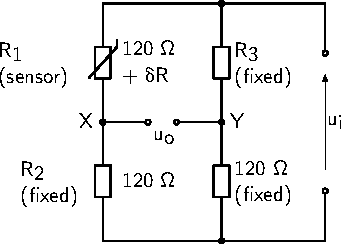
\includegraphics[scale=0.9]{fig/lec03/wheatstone_DC_bridge.pdf}
    \caption*{Wheatstone Bridge Circuit}
\end{figure}
\end{columns}

\textbf{Use cases:}  
Strain gauges, RTDs, precision resistance measurement.  
\textbf{Advantages:} simple, accurate, high SNR.  
\textbf{Disadvantages:} 4-resistor matching needed, temp-drift.
\end{frame}

\begin{frame}{Practical Wheatstone Bridge with Zero \& Sensitivity Adjustments}
\small
\begin{columns}
\column{0.55\textwidth}
\begin{itemize}
    \item Variable resistor $R_4$ used for \textbf{zero adjustment}.
    \item $R_S$ introduces \textbf{sensitivity control} for the null detector.
\end{itemize}

\textbf{Output near balance:}
\[
e_o \approx \frac{e_i}{4R}( \Delta R_1 - \Delta R_3 )
\]

\textbf{Use cases:}  
Industrial load cells, pressure transducers, torque sensors.

\column{0.45\textwidth}
\begin{figure}
    \centering
    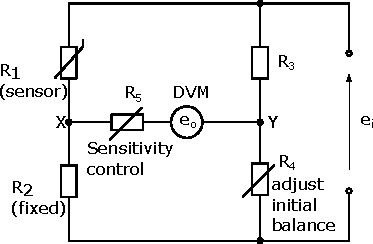
\includegraphics[scale=0.9]{fig/lec03/modi_wheatstone_DC_bridge.pdf}
    \caption*{Practical Wheatstone Bridge Circuit}
\end{figure}
\end{columns}
\end{frame}



\begin{frame}{Double Active Arm Bridge (Two-Element Bridge)}
\small
\begin{columns}
\column{0.55\textwidth}

\textbf{Purpose:} Increase sensitivity + temperature compensation.

\[
e_o \approx \frac{e_i}{2R}(\Delta R)
\]

\textbf{Advantages:}
\begin{itemize}
    \item Doubles output sensitivity.
    \item Self-temperature-compensating.
\end{itemize}

\textbf{Use cases:}  
Mechanical systems with tension/compression pairs (e.g., 4-arm strain gauge load cells).

\column{0.45\textwidth}
\begin{figure}
    \centering
    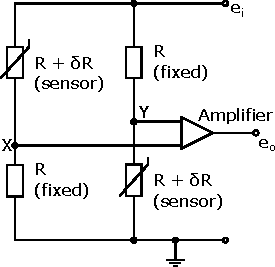
\includegraphics[scale=0.9]{fig/lec03/two_sensitive_bridge.pdf}
    \caption*{Double Active Arm Bridge Circuit}
\end{figure}
\end{columns}
\end{frame}


\begin{frame}{Full Bridge with Four Active Sensors}
\small
\textbf{Maximum sensitivity:}
\[
e_o = \frac{e_i}{4} \left( \frac{\Delta R}{R} \right) \times 4
\]

\textbf{Advantages:}
\begin{itemize}
    \item Highest output level.
    \item Excellent common-mode rejection.
    \item Full temperature compensation.
\end{itemize}

\textbf{Use cases:} high-accuracy weighing systems, multi-axis force sensors.

\end{frame}


\begin{frame}{General AC Bridge Theory}
\small

\begin{columns}
\column{0.5\textwidth}
\textbf{Impedance representation:}
\[
Z = R + jX, \qquad [Z\ \Omega]
\]

\textbf{Balance condition:}
\[
Z_1 Z_4 = Z_2 Z_3
\]

\textbf{For balance:}
\begin{itemize}
    \item Real parts must match.
    \item Imaginary parts must match.
\end{itemize}

\textbf{Use cases:}  
Inductance, capacitance, dielectric loss, dissipation factor.
\column{0.5\textwidth}
\begin{figure}
    \centering
    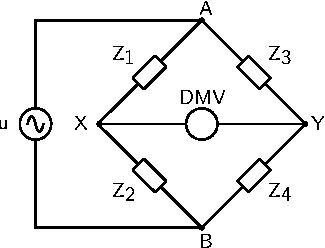
\includegraphics[scale=0.9]{fig/lec03/four_active_bridge.pdf}
    \caption*{General AC Bridge Circuit}
\end{figure}
\end{columns}
\end{frame}

% ----------------------------------------------------------
\begin{frame}{Maxwell Bridge (Inductance with Resistance)}
\small
\begin{columns}
\column{0.65\textwidth}
\textbf{Used for:} measuring inductance $L$ in series with resistance $R$.

\[
Z_1 = \frac{R_1}{1 + j\omega R_1 C_1}
\quad
Z_4 = R_4 + j\omega L_4
\]

\textbf{From balance:}
\[
R_4 = \frac{R_2 R_3}{R_1}, \qquad [\Omega]
\]
\[
L_4 = R_2 R_3 C_1, \qquad [\text{H}]
\]

\textbf{Advantages:}
\begin{itemize}
    \item Frequency-independent solution.
    \item Easy to balance physically.
\end{itemize}

\textbf{Disadvantages:} not suitable for high-Q coils.  
\textbf{Use cases:} medium inductors (10 mH–100 H).
\column{0.35\textwidth}
\begin{figure}
    \centering
    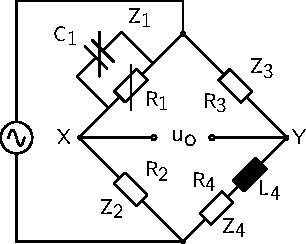
\includegraphics[scale=0.9]{fig/lec03/maxwell.pdf}
    \caption*{Maxwell Bridge Circuit}
\end{figure}
\end{columns}
\end{frame}

% ----------------------------------------------------------
\begin{frame}{Hay Bridge (High-Q Inductance Measurement)}
\small
\begin{columns}
\column{0.65\textwidth}
\textbf{Used for:} inductors with small series resistance (high Q).

\[
R_1 R_4 = R_2 R_3, \qquad [\Omega]
\]
\[
L_4 = R_2 R_3 C_1, \qquad [\text{H}]
\]

\textbf{Advantages:}
\begin{itemize}
    \item Works well for high-Q inductors.
    \item Frequency-independent result.
\end{itemize}

\textbf{Disadvantages:}  
Not accurate for lossy inductors.
\column{0.35\textwidth}
\begin{figure}
    \centering
    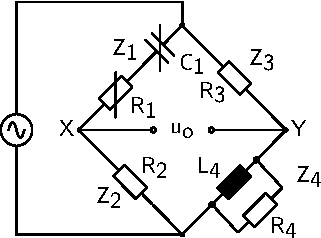
\includegraphics[scale=0.9]{fig/lec03/hay_bridge.pdf}
    \caption*{Hay Bridge Circuit}
\end{figure}
\end{columns}

\end{frame}

% ----------------------------------------------------------
\begin{frame}{Schering Bridge (Capacitance + Loss Measurement)}
\small
\begin{columns}
\column{0.6\textwidth}
\textbf{Unknown:} $C_4$ with series loss $R_4$.

\[
R_1 C_3 = R_2 C_4 \qquad [\text{s}]
\]
\[
R_4 C_4 = R_1 C_1
\]

\textbf{Measures:}
\begin{itemize}
    \item Capacitance $C$ (in farads)
    \item Dissipation factor, dielectric loss
\end{itemize}

\textbf{Use cases:} insulation testing, high-voltage apparatus, dielectric materials.

\column{0.4\textwidth}
\begin{figure}
    \centering
    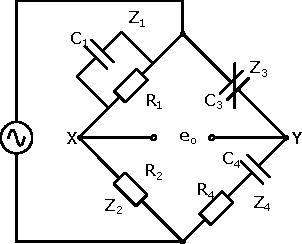
\includegraphics[scale=0.9]{fig/lec03/schering_bridge.pdf}
    \caption*{Schering Bridge Circuit}
\end{figure}
\end{columns}

\end{frame}

\begin{frame}{The Wien Frequency Bridge: Principle and Circuit}
\small
\begin{columns}
\column{0.65\textwidth}
\textbf{Purpose:}  
The Wien frequency bridge is designed so that the bridge balances (i.e., $e_o = 0$) \textbf{only at one specific frequency} of the applied AC signal.  
Thus, it acts as a \textbf{notch filter} or a selective frequency measurement circuit.

\textbf{Circuit characteristics:}
\begin{itemize}
    \item Arms $Z_3$ and $Z_4$ are pure resistances, with $Z_4 = 2 Z_3$.
    \item Variable resistors $R_1$ and $R_2$ are mechanically ganged so both adjust simultaneously to the same value $R$.
    \item Capacitors in opposite arms $C_1$ and $C_2$ have identical values $C$.
\end{itemize}

\textbf{Impedances:}
\[
Z_1 = \frac{R}{1 + j\omega C R}, \qquad
Z_2 = R + \frac{1}{j\omega C}
\]
\[
Z_3 = R_3 \qquad\qquad
Z_4 = 2R_3
\]
\column{0.35\textwidth}

\begin{figure}
    \centering
    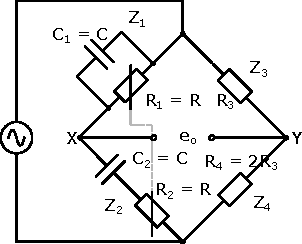
\includegraphics[scale=0.9]{fig/lec03/wein_bridge.pdf}
    \caption*{Wien Frequency Bridge Circuit}  
\end{figure}
\end{columns}

\end{frame}


\begin{frame}{Wien Frequency Bridge: Balance Condition and Frequency}
\small
\begin{columns}
\column{0.65\textwidth}
\textbf{Balance condition for AC bridges:}
\[
Z_1 Z_4 = Z_2 Z_3
\]

Substitute impedances:
\[
\frac{R}{1 + j\omega CR} \cdot 2R_3 
= 
\left(R + \frac{1}{j\omega C}\right) R_3
\]

After simplifying and separating real and imaginary parts, the balance occurs when:
\[
\omega = \frac{1}{CR} \quad [\mathrm{rad/s}]
\]
\[
f = \frac{1}{2\pi CR} \quad [\mathrm{Hz}]
\]
\column{0.35\textwidth}
\begin{figure}
    \centering
    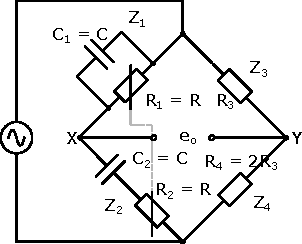
\includegraphics[scale=0.9]{fig/lec03/wein_bridge.pdf}
    \caption*{Wien Frequency Bridge Circuit}
\end{figure}

\end{columns}
\end{frame}



\begin{frame}{Wien Frequency Bridge: Balance Condition and Frequency}
\small
\begin{columns}
\column{0.65\textwidth}
\textbf{Interpretation:}
\begin{itemize}
    \item Bridge gives \textbf{zero output} only at a single frequency.
    \item Acts as a \textbf{precise frequency indicator} or \textbf{notch filter}.
\end{itemize}

\textbf{Advantages:}
\begin{itemize}
    \item High frequency selectivity.
    \item Components adjust symmetrically → good stability.
\end{itemize}

\textbf{Limitations:}
\begin{itemize}
    \item Sensitive to tolerance of $R$ and $C$.
    \item Not suitable for broadband measurements.
\end{itemize}
\column{0.35\textwidth}
\begin{figure}
    \centering
    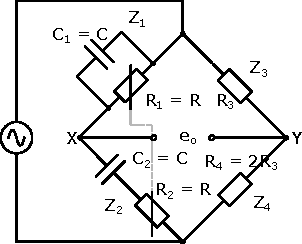
\includegraphics[scale=0.9]{fig/lec03/wein_bridge.pdf}
    \caption*{Wien Frequency Bridge Circuit}
\end{figure}

\end{columns}
\end{frame}


\begin{frame}{Summary Table: DC and AC Bridges}
\small
\begin{tabular}{p{2.5cm} p{4.5cm} p{4cm}}
\toprule
\textbf{Bridge} & \textbf{Measures} & \textbf{Use Cases} \\
\midrule
Wheatstone & Resistance, $\Delta R$ & Strain, RTD \\
Practical Wheatstone & Precise $\Delta R$ & Load cells \\
Double-arm bridge & High sensitivity & Force/torque \\
Maxwell & L with R & Medium inductors \\
Hay & High-Q inductors & RF coils \\
Schering & C and dielectric loss & HV equipment \\
Maxwell–Wien & Precision L & Standards \\
De Sauty & Ideal C & Cap. comparison \\
Owen & Low-Q inductors & Lossy coils \\
Wien frequency & Frequency $f$ & Oscillators \\
\bottomrule
\end{tabular}
\end{frame}

\begin{frame}{Introduction to Operational Amplifiers}
\small
\textbf{Why Op-Amps?}
\begin{itemize}
    \item Widely used in analog signal conditioning, filtering, instrumentation, and measurement systems.
    \item Originally used in analog computers for mathematical operations: 
    addition, subtraction, differentiation, integration.
    \item Modern op-amps are compact ICs with high performance, low noise, and wide bandwidth.
\end{itemize}

\textbf{Role in Signal Conditioning}
\begin{itemize}
    \item Amplification of weak sensor signals.
    \item Conversion between signal domains (e.g., current–voltage).
    \item Implementation of filters and mathematical operations.
    \item Isolation between high/low impedance stages.
\end{itemize}
\end{frame}


\begin{frame}{Operational Amplifier Terminals}
\small
\begin{columns}
\column{0.5\textwidth}
\textbf{Terminals of an Op-Amp}
\begin{itemize}
    \item Two input terminals: 
    \begin{itemize}
        \item Non-inverting input ($+$)
        \item Inverting input ($-$)
    \end{itemize}
    \item One output terminal.
\end{itemize}

\textbf{Input Configurations}
\begin{itemize}
    \item Single-ended input and output.
    \item Differential input, single-ended output.
    \item Differential input and differential output.
\end{itemize}

\column{0.5\textwidth}
\begin{figure}
    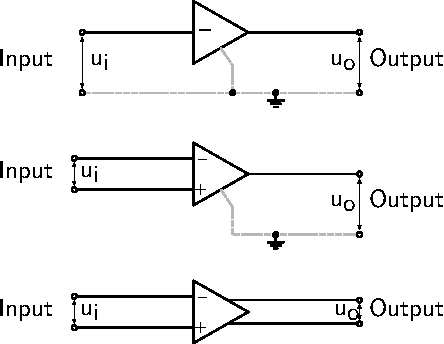
\includegraphics[width=0.75\linewidth]{fig/lec03/op_amp_sym.pdf}
    \caption*{Op-amp configurations: single-ended and differential}
\end{figure}
\end{columns}
\end{frame}

\begin{frame}{Characteristics of the Ideal Operational Amplifier}
\small
An ideal op-amp is defined by the following properties:

\begin{enumerate}
    \item \textbf{Infinite open-loop gain}, $A_{\mathrm{VOL}} \rightarrow \infty$
    \item \textbf{Infinite input impedance}, $Z_{\mathrm{in}} \rightarrow \infty$  
    $\rightarrow$ No input current: $i_+ = i_- = 0$
    \item \textbf{Zero output impedance}, $Z_{\mathrm{out}} = 0$
    \item \textbf{Infinite bandwidth}  
    $\rightarrow$ constant gain from DC to $\infty$
    \item \textbf{Zero input offset voltage and current}
\end{enumerate}

\textbf{Implications:}
\begin{itemize}
    \item No voltage difference between inputs under negative feedback.
    \item Output adjusts to maintain $v_+ = v_-$.
\end{itemize}
\end{frame}

\begin{frame}{Golden Rules of Ideal Op-Amps}
\small
\begin{columns}
\column{0.6\textwidth}

\textbf{Golden Rule 1:}  
Under negative feedback, the op-amp forces  
\[
v_+ = v_-
\]

\textbf{Golden Rule 2:}  
\[
i_+ = i_- = 0
\]
No current flows into either input terminal.

\textbf{Consequences:}
\begin{itemize}
    \item The inverting input can act as a \textbf{virtual ground} if the non-inverting terminal is grounded.
    \item The inverting node becomes a \textbf{summing point} for currents.
\end{itemize}
\column{0.4\textwidth}
\begin{figure}
    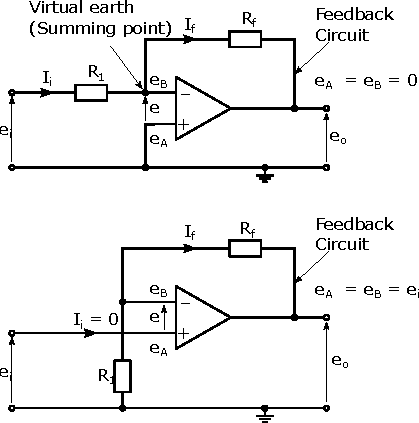
\includegraphics[width=0.7\linewidth]{fig/lec03/basic_op_amp.pdf}
    \caption*{Inverting and non-inverting feedback configurations}
\end{figure}
\end{columns}
\end{frame}


\begin{frame}{Inverting Operational Amplifier}
\small
\begin{columns}
\column{0.65\textwidth}

\textbf{Circuit Principle}
\begin{itemize}
    \item Input applied to the inverting terminal via resistor $R_i$.
    \item Feedback resistor $R_f$ returns output to inverting input.
    \item Non-inverting terminal grounded ($v_+=0$).
\end{itemize}

\textbf{Derivation}
Using Golden Rules:
\[
i_i = \frac{e_i}{R_i}, \quad i_f = \frac{-e_o}{R_f}
\]
Since $i_i = i_f$:
\[
\frac{e_i}{R_i} = -\frac{e_o}{R_f}
\]
\[
\Rightarrow \frac{e_o}{e_i} = -\frac{R_f}{R_i}
\]


\column{0.35\textwidth}
\begin{figure}
\hspace{-1cm}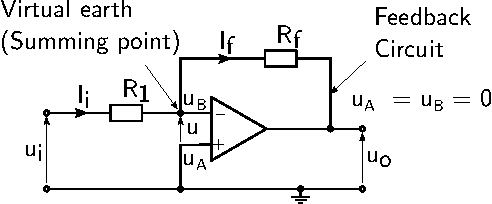
\includegraphics[scale=0.8]{fig/lec03/invert_op_amp.pdf}
\end{figure}
\textbf{Closed-loop gain:}
\[
A_{V,CL} = -\frac{R_f}{R_i}
\]
\end{columns}
\end{frame}


\begin{frame}{Non-Inverting Operational Amplifier}
\small
\begin{columns}
\column{0.65\textwidth}


\textbf{Key Feature:} Input is applied to the $+$ terminal, so output is in-phase.

\[
e_B = e_i
\]

Using feedback current:
\[
i_f = \frac{0 - e_o}{R_1 + R_f}
\]

From nodal condition:
\[
i_f = \frac{e_i - e_o}{R_f}
\]

Solving the equations:
\[
A_{V,CL} = \frac{e_o}{e_i} = 1 + \frac{R_f}{R_i}
\]



\column{0.35\textwidth}
\begin{figure}
\hspace{-1cm}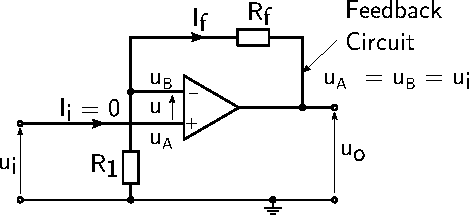
\includegraphics[scale=0.8]{fig/lec03/non_invert_op_amp.pdf}
\end{figure}
\textbf{Properties:}
\begin{itemize}
    \item No inversion of signal.
    \item High input impedance.
\end{itemize}
\end{columns}
\end{frame}


\begin{frame}{Op-Amp as a Current-to-Voltage Converter}
\small
\begin{columns}
\column{0.6\textwidth}

\textbf{Used in:}
\begin{itemize}
    \item Photodiodes
    \item Sensors generating current output
    \item Precision current measurement
\end{itemize}

\textbf{Derivation:}
Current flows through $R_f$:
\[
e_o = - I_i R_f \quad \text{(V)}
\]

\textbf{Units:}  
$[I_i]=$ A, $[R_f]=$ $\Omega$, $[e_o]=$ V

\column{0.4\textwidth}
\begin{figure}
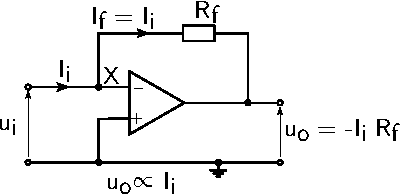
\includegraphics[width=1\linewidth]{fig/lec03/current_to_voltage.pdf}
\end{figure}
\end{columns}
\end{frame}

\begin{frame}{Summing Amplifier (Current Summation)}
\small
\begin{columns}
\column{0.5\textwidth}

\textbf{Currents summed at virtual ground:}
\[
I_f = I_1 + I_2 + I_3
\]

Output:
\[
e_o = -R_f(I_1 + I_2 + I_3)
\]

\textbf{Voltage Summation Form:}
\[
e_o = -R_f\left(\frac{e_1}{R_1} + \frac{e_2}{R_2} + \frac{e_3}{R_3}\right)
\]

\column{0.5\textwidth}
\begin{figure}
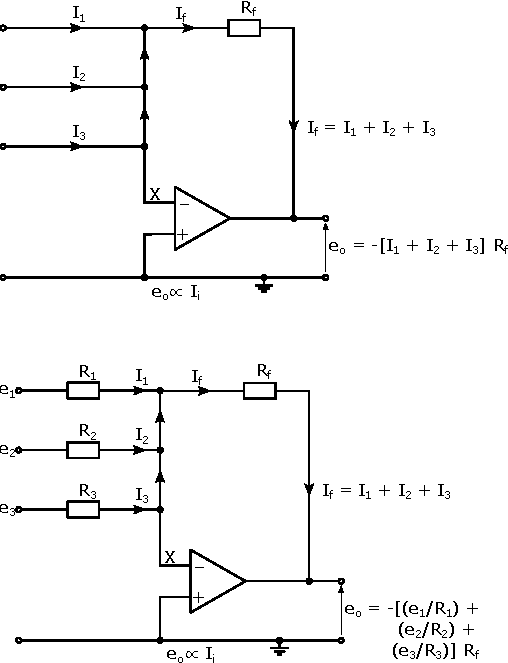
\includegraphics[width=0.7\linewidth]{fig/lec03/summing_amplifier.pdf}
\end{figure}
\end{columns}
\end{frame}

\begin{frame}{Voltage-to-Current Converter (V-I Converter)}
\small
\begin{columns}
\column{0.4\textwidth}

\[
I_L = \frac{e_i}{R_1}
\]

\textbf{Load current independent of load resistor:}  
Set by $R_1$ only.

Used in:
\begin{itemize}
    \item Actuators
    \item Transducer excitation
    \item Analog driving circuits
\end{itemize}

\column{0.6\textwidth}
\begin{figure}
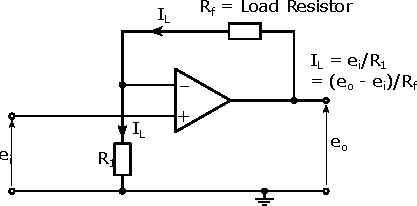
\includegraphics[width=0.6\linewidth]{fig/lec03/volt_to_current.pdf}
\end{figure}
\end{columns}
\end{frame}


\begin{frame}{Op-Amp as a Buffer (Voltage Follower)}
\small
\begin{columns}
\column{0.4\textwidth}

\textbf{Unity gain:}
\[
e_o = e_i
\]

\textbf{Purpose:}
\begin{itemize}
    \item High input impedance.
    \item Low output impedance.
    \item Prevents loading of previous stage.
\end{itemize}

\column{0.6\textwidth}
\begin{figure}
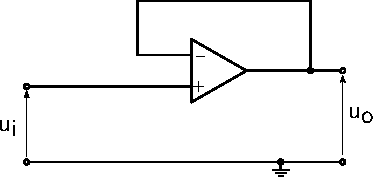
\includegraphics[width=0.6\linewidth]{fig/lec03/buffer.pdf}
\end{figure}
\end{columns}
\end{frame}

\begin{frame}{Ideal Op-Amp Differential Subtractor}
\small
\begin{columns}
\column{0.4\textwidth}
\textbf{Deriving the Output Voltage:}
\[
 e_1 \frac{R_2}{R_T}
 = e_2 \frac{R_2}{R_T} + e_o \frac{R_1}{R_T}
\]
Cancel $R_T$ (=$R_1$ + $R_2$) and rearrange:
\[
   e_o = (e_1 - e_2)\frac{R_2}{R_1}
\]

\vspace{6pt}
\textbf{Final Transfer Function:}
\[
\boxed{
e_o = (e_1 - e_2)\frac{R_2}{R_1}
}
\]

\column{0.6\textwidth}
\begin{figure}
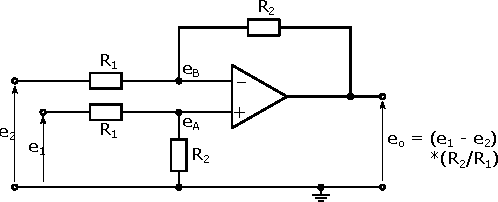
\includegraphics[width=0.6\linewidth]{fig/lec03/differential.pdf}
\end{figure}
\textbf{Output expression:}
\[
e_o = (e_1 - e_2)\frac{R_2}{R_1}
\]

\textbf{Use Cases:}
\begin{itemize}
    \item Sensor differential measurement.
    \item Rejecting common-mode interference.
\end{itemize}
\end{columns}
\end{frame}

\begin{frame}{Ideal Op-Amp Integrator}
\small
%\vspace{-0.5cm}
\begin{columns}
\column{0.6\textwidth}
Input current through $R$:
\[
   I_i = \frac{e_i(t) - 0}{R} = \frac{e_i(t)}{R} \quad [\si{\ampere}]
\]
Feedback current through capacitor $C$ (voltage across $C$ is $v_C = -e_o(t)$):
\[
   I_f = C \, \frac{\mathrm{d}v_C}{\mathrm{d}t}
       = C \, \frac{\mathrm{d}(-e_o(t))}{\mathrm{d}t}
       = -C \, \frac{\mathrm{d}e_o(t)}{\mathrm{d}t}
\]

Equating $I_i = I_f$:
\[
   \frac{e_i(t)}{R} = -C \, \frac{\mathrm{d}e_o(t)}{\mathrm{d}t}
\]

\textbf{Output–input relationship (integrator equation):}
\[
   \frac{\mathrm{d}e_o(t)}{\mathrm{d}t} = -\frac{1}{RC} e_i(t)
   \quad \Longrightarrow \quad
   e_o(t) = -\frac{1}{RC} \int e_i(t)\,\mathrm{d}t + e_o(0)
\]

\column{0.4\textwidth}
\begin{figure}
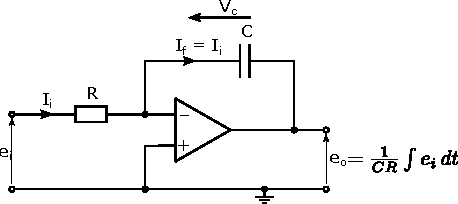
\includegraphics[width=0.8\linewidth]{fig/lec03/integrator.pdf}
\end{figure}
For a properly reset integrator with $e_o(0)=0$:
\[
\boxed{
   e_o(t) = -\dfrac{1}{RC} \displaystyle\int e_i(t)\,\mathrm{d}t
}
\]
with $R$ in \si{\ohm}, $C$ in \si{\farad}, so $RC$ has units of \si{\second}.

\end{columns}
\end{frame}

\begin{frame}{Ideal Operational Amplifier as a Differentiator}
\small
\begin{columns}
\column{0.5\textwidth}
\textbf{Concept:}
\begin{itemize}
    \item A differentiator produces an output proportional to the \textbf{time derivative} of the input voltage.
    \item Achieved by interchanging the feedback resistor and input capacitor of the integrator circuit.
    \item Uses \textbf{inverting} op-amp configuration.
\end{itemize}
\textbf{Derivation:}
\begin{align*}
    i_i &= C \frac{d e_i}{dt} \\
    i_f &= \frac{-e_o}{R} \\
    i_i &= i_f \quad \\
    C \frac{d e_i}{dt} &= -\frac{e_o}{R}
\end{align*}
\column{0.5\textwidth}
\begin{figure}
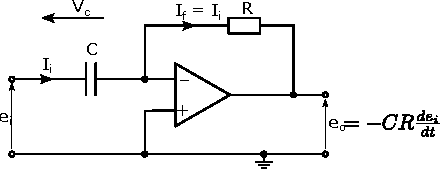
\includegraphics[width=0.7\linewidth]{fig/lec03/differentiator.pdf}
\end{figure}
\textbf{Output Voltage:}
\[
    \boxed{
    e_o = - C R \frac{d e_i}{dt}
    }
\]
\end{columns}

\end{frame}

\begin{frame}{Ideal Operational Amplifier as a Differentiator}
    \small
\textbf{Characteristics:}
\begin{itemize}
    \item \textbf{Gain factor:} $CR$ (units: \si{\second})
    \item Output leads input by \SI{90}{\degree} in phase for sinusoidal signals.
\end{itemize}

\textbf{Advantages:}
\begin{itemize}
    \item Ideal for edge detection and high-frequency transient measurement.
    \item Produces sharp spikes for fast changes in input.
\end{itemize}

\textbf{Limitations (Practical):}
\begin{itemize}
    \item Highly sensitive to high-frequency noise (since noise has large derivatives).
    \item Real circuits require a small series resistor with $C$ and RC stabilisation.
\end{itemize}

\textbf{Applications:}
\begin{itemize}
    \item Signal processing: differentiation of waveforms.
    \item Edge/transition detection (square $\rightarrow$ impulse).
    \item Analog computing, PID controllers (derivative term).
\end{itemize}

\end{frame}

\begin{frame}{Summary of Op-Amp Configurations}
\small
\begin{tabular}{p{3cm} p{5cm} p{5cm}}
\toprule    
\textbf{Configuration} & \textbf{Transfer Function} & \textbf{Use Cases} \\
\midrule    
Inverting Amplifier & $e_o = -\frac{R_f}{R_i} e_i$ & Signal inversion, amplification \\
Non-Inverting Amplifier & $e_o = \left(1 + \frac{R
_f}{R_i}\right) e_i$ & Buffering, high input impedance \\
Current-to-Voltage Converter & $e_o = -I_i R_f$ & Photodiodes, current sensors \\
Summing Amplifier & $e_o = -R_f\left(\frac{e_1}{R_1} + \frac{e_2}{R_2} + \ldots\right)$ & Audio mixing, sensor fusion \\
Voltage-to-Current Converter & $I_L = \frac{e_i}{R_1}$ & Actuator driving, transducer excitation \\
Buffer (Voltage Follower) & $e_o = e_i$ & Impedance matching, isolation \\
Differential Subtractor & $e_o = (e_1 - e_2)\frac   {R_2}{R_1}$ & Differential measurement, noise rejection \\
Integrator & $e_o(t) = -\frac{1}{RC} \int e_i(t)\,dt$ & Signal integration, analog computing \\
Differentiator & $e_o = -CR \frac{d e_i}{dt}$ & Edge detection, transient analysis \\
\bottomrule 
\end{tabular}
\end{frame}

\begin{frame}{Operational Amplifier Frequency Response}
\small

\textbf{Key idea:} The practical operational amplifier does \emph{not} respond instantaneously to an input signal.  
Finite internal compensation introduces a \textbf{delay} and \textbf{frequency-dependent gain}.

\begin{itemize}
    \item At \textbf{low frequencies (DC – few Hz)}, delay is negligible.
    \item At \textbf{higher frequencies}, finite gain-bandwidth causes:
    \begin{itemize}
        \item magnitude drop (gain roll-off),
        \item phase lag between input and output,
        \item distortion for large-signal or fast-changing inputs.
    \end{itemize}
    \item Therefore, analysis uses only \textbf{small-signal sinusoidal} inputs.
\end{itemize}

\textbf{Model:}  
For many op-amps, the open-loop transfer function is:
\[
A_{OL}(j f) = \frac{A_{OL}}{1 + j\frac{f}{f_c}}
\]
where:
\[
A_{OL} \text{ (DC gain)},\quad f_c \text{ (break frequency in Hz)}
\]

\end{frame}


\begin{frame}{Voltage Gain in Decibels}
\small

\begin{columns}
\column{0.6\textwidth}
For sinusoidal steady-state, the gain is expressed in \textbf{decibels (dB)} as:

\[
G_{\mathrm{dB}} = 20 \log_{10}\left(\frac{e_o}{e_i}\right)
\]

\textbf{Interpretation:}
\begin{itemize}
    \item Negative dB → attenuation.
    \item Positive dB → amplification.
    \item Note: \emph{Power} is proportional to voltage squared → doubling power corresponds to $+3$ dB.
\end{itemize}

\textbf{Example table values:}

\begin{itemize}
    \item $e_o/e_i = 1$ → $0$ dB → unity gain.
    \item $e_o/e_i = 10$ → $20$ dB.
    \item $e_o/e_i = 0.5$ → $-6$ dB → quarter power.
\end{itemize}
\column{0.4\textwidth}
\begin{table}[h!]
\centering
\caption{Voltage ratio and decibel relationship}
\label{tab:voltage_ratio_db}
\begin{tabular}{ccc}
\toprule
$\dfrac{e_o}{e_i}$ & dB & Power output \\
\midrule
0.1   & $-20$ &  \\
0.5   & $-6$  & Quarter \\
0.707 & $-3$  & Half \\
1     & $0$   & Unity \\
1.41  & $3$   & Double \\
2     & $6$   &  \\
10    & $20$  &  \\
100   & $40$  &  \\
\bottomrule
\end{tabular}
\end{table}
\end{columns}

\end{frame}


\begin{frame}{Complex Gain Representation and Phase Lag}
\small
\begin{columns}
\column{0.65\textwidth}

Amplifier gain is a \textbf{complex quantity}:
\[
A = |A| e^{j\theta}
\]

A sinusoidal signal can be expressed as:
\[
r = x + j y, \qquad |r| = \sqrt{x^2 + y^2},\qquad \theta = \tan^{-1}\left(\frac{y}{x}\right)
\]

\textbf{Importance:}
\begin{itemize}
    \item Phase lag increases with frequency.
    \item Causes reduction in stability (important for feedback design).
\end{itemize}

\column{0.35\textwidth}
\begin{figure}[h]
\centering
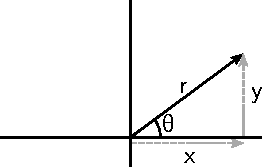
\includegraphics[width=1\linewidth]{fig/lec03/complex_representation.pdf} 
\end{figure}

\end{columns}
\end{frame}

\begin{frame}{Bode Plot for Op-Amp Magnitude Response}
\small
\begin{columns}
\column{0.35\textwidth}

Open-loop magnitude response:
\[
|A_{OL}(jf)| = \frac{A_{OL}}{\sqrt{1 + \left(\frac{f}{f_c}\right)^2}}
\]

\textbf{Key points:}
\begin{itemize}
    \item For $f \ll f_c$: gain $\approx A_{OL}$
    \item For $f = f_c$: gain drops by \textbf{3 dB}
    \item For $f \gg f_c$: gain falls with slope \textbf{20 dB/decade}
    \item At unity-gain frequency $f_1$: $|A| = 1$ or $0$ dB
\end{itemize}

\column{0.65\textwidth}
\begin{figure}[h]
\centering
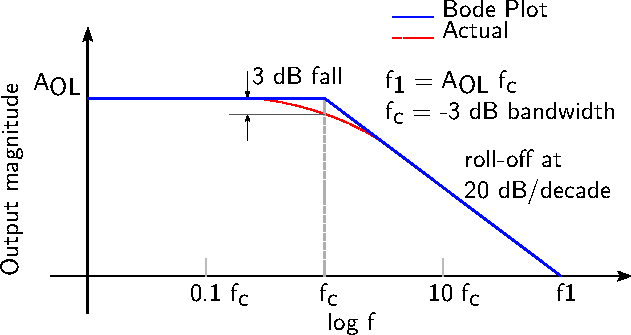
\includegraphics[width=0.8\linewidth]{fig/lec03/freq_mag.pdf}
\end{figure}
\end{columns}
\end{frame}

\begin{frame}{Bode Plot for Op-Amp Phase Response}
\small
\begin{columns}
\column{0.35\textwidth}

Phase shift for single-pole op-amp:
\[
\theta(f) = -\tan^{-1}\left(\frac{f}{f_c}\right)
\]

\textbf{Important values:}
\begin{itemize}
    \item At $f = 0$: $\theta = 0^\circ$
    \item At $f = f_c$: $\theta = -45^\circ$
    \item At $f \gg f_c$: $\theta \rightarrow -90^\circ$
\end{itemize}

\column{0.65\textwidth}
\begin{figure}[h]
\centering
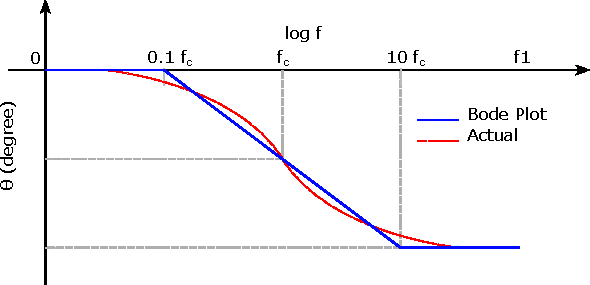
\includegraphics[width=1\linewidth]{fig/lec03/phase.pdf}
\end{figure}
\end{columns}
\end{frame}

\begin{frame}{Break Frequency and Unity-Gain Frequency}
\small

\textbf{Break frequency} $f_c$:  
Point where open-loop gain drops by \SI{3}{\decibel}.

\[
f_c = \frac{1}{2\pi R C} \quad \text{(for internally compensated op-amp)}
\]

\textbf{Unity-gain frequency} $f_1$:
\[
A_{OL}(f_1) = 1
\]

\[
f_1 \approx A_{OL} \cdot f_c
\]

\textbf{Implications:}
\begin{itemize}
    \item Sets maximum usable closed-loop bandwidth.
    \item Determines speed/slew performance.
\end{itemize}

\end{frame}


\begin{frame}{Why Frequency Response Matters in Practice}
\small

\textbf{1. Stability considerations}
\begin{itemize}
    \item Large phase lags $\rightarrow$ risk of oscillations in feedback systems.
    \item Phase margin must be $>$ $45^\circ$ for robustness.
\end{itemize}

\textbf{2. Closed-loop bandwidth limitations}
\[
\text{Closed-loop bandwidth} \approx \frac{f_1}{\text{Closed-loop gain}}
\]

\textbf{3. Accuracy and distortion}
\begin{itemize}
    \item High frequencies → increased error.
    \item Important for instrumentation and fast control loops.
\end{itemize}

\textbf{4. Noise performance}
\begin{itemize}
    \item Noise increases at high frequency.
    \item Filtering and layout become critical.
\end{itemize}

\end{frame}


\begin{frame}{Linear Scaling Circuits} %This should be moved in the start of the lecture of operational amplifiers.
\small
\begin{itemize}
    \item Linear scaling circuits produce an output $e_o$ that is a linear function of input $e_i$:
    \[
        e_o = f(e_i) = m e_i + c
    \]
    where:
    \begin{itemize}
        \item $m$ — slope or gain (dimensionless)
        \item $c$ — output offset at zero input (V)
    \end{itemize}

    \item Linear behaviour implies:
    \begin{itemize}
        \item Proportional change in output for change in input.
        \item No distortion or frequency dependence (requires purely resistive components).
    \end{itemize}

    \item Applications:
    \begin{itemize}
        \item Voltage scaling (amplification/attenuation)
        \item Impedance conversion
        \item Signal addition/subtraction
        \item Voltage-to-current or current-to-voltage conversion
    \end{itemize}
\end{itemize}
\end{frame}

\begin{frame}{Graphical Interpretation of Linearity}
\small
\begin{columns}
\column{0.5\textwidth}
\begin{itemize}
    \item Linear circuits maintain a straight-line $e_o$–$e_i$ relationship.
    \item Examples with positive and negative slopes.
\end{itemize}

\[
    \frac{\Delta e_o}{\Delta e_i} = m
\]
\column{0.5\textwidth}
\begin{figure}
    \centering
    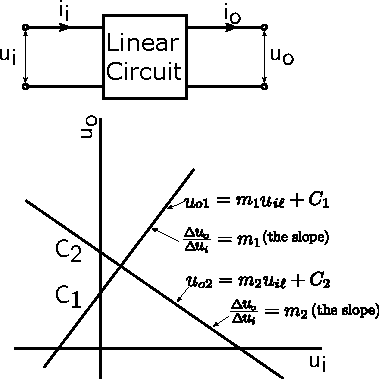
\includegraphics[width=0.75\linewidth]{fig/lec03/linear_ckts.pdf}
    \caption*{Linear $e_o$ vs. $e_i$ relationships}
\end{figure}
\end{columns}

\end{frame}

\begin{frame}{Design Requirements}
\small
\begin{itemize}
    \item Circuit must behave identically over relevant frequency range $\rightarrow$ resistive components essential.

    \item Selection of resistor values:
    \begin{itemize}
        \item Must avoid loading the sensor/source.
        \item Should not be extremely large (bias current → offset errors).
        \item Should not be extremely small (excess current loading).
    \end{itemize}

    \item General-purpose op-amps require minimum output load:
    \[
        R_L \geq 2\;\text{k}\Omega (\text{check datasheet!})
    \]

    \item In inverting amplifiers, input resistor $R_1$ determines input impedance:
    \[
        Z_{\text{in}} = R_1
    \]
    \item High-precision resistors (0.1\% tolerance or better) recommended for accuracy.
    \item Common examples are: inverting/non-inverting amplifiers, summing amplifiers, voltage/current converters, buffers that we learnt in previous slides.
\end{itemize}
\end{frame}


\begin{frame}
{Summary}
\begin{itemize}
    \item In summary, linear scaling circuits using op-amps provide precise control over signal amplitude and offset.
    \item Proper design ensures minimal loading, high accuracy, and stable operation across the desired frequency range.
    \item These circuits form the foundation for more complex signal conditioning and processing tasks in instrumentation systems.
    \item There are topics related to non linear circuits and other advanced op-amp configurations that can be explored at your end based on interest.
    \item This concludes our discussion on introduction of using operational amplifiers.
\end{itemize}
\end{frame}


%=====================================================
\begin{frame}{Transducer Amplifiers: Overview}
\textbf{Transducers} convert one form of energy into another. In instrumentation systems, we often use transducers that convert a physical stimulus into an electrical quantity.

\vspace{0.2cm}
Common resistive transducers:
\begin{itemize}
    \item Strain gauges
    \item Resistance thermometers (RTDs)
    \item Thermistors
    \item Potentiometric transducers
    \item Light-dependent resistors (LDRs)
\end{itemize}

\vspace{0.2cm}
Most resistive transducers are used inside a \textbf{Wheatstone bridge}. When the transducer resistance changes by a small fraction, the bridge becomes unbalanced and generates a measurable voltage.

\vspace{0.2cm}
\textbf{Goal}: Amplify this small differential voltage to a useful level using an operational amplifier.

\end{frame}

%=====================================================
\begin{frame}{Bridge Amplifier}
\begin{itemize}
    \item The transducer element has resistance \(R_X = R(1+a)\), where \(a\) is a small fractional change.
    \item Bridge is biased by supply \(E\), with opposite corners labelled X and Y.
    \item The op-amp forces its input nodes to the same potential: \(V_X = V_Y = V\).
    \item Small imbalance is converted into output voltage \(e_o\).
\end{itemize}
\begin{columns}
\column{0.55\textwidth}
At node X:
\begin{equation*}
\frac{E - V_X}{R} = \frac{V_X - e_o}{R_f} + \frac{V_X}{R} 
\end{equation*}
At node Y:
\begin{equation*}
\frac{E - V_Y}{R} = \frac{V_Y}{R(1+a)} + \frac{V_Y}{R_f}
\end{equation*}
Because the op-amp forces \(V_X = V_Y = V\), the above can be combined to yield the bridge output relation:
\column{0.45\textwidth}
\vspace{-1cm}
\begin{figure}
    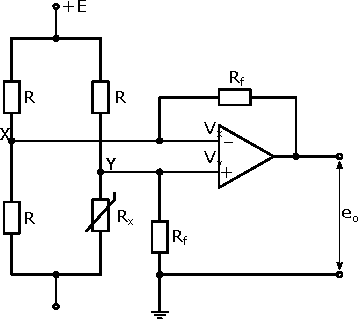
\includegraphics[width=0.7\linewidth]{fig/lec03/bridge_amp.pdf}
    \caption*{Bridge amplifier with resistive transducer}
\end{figure}
\vspace{-0.5cm}
\begin{equation*}
e_o = \left[ \frac{V}{R} - \frac{V}{R(1+a)} \right] R_f
\end{equation*}
\end{columns}
\end{frame}

%=====================================================
\begin{frame}{Bridge Amplifier: Solving for Output}
From analysis of the right-hand side of the bridge:
\begin{columns}
\column{0.5\textwidth}
\begin{equation*}
V = V_Y = E \left[ \frac{R(1+a) \parallel R_f}{R + (R(1+a) \parallel R_f)} \right]
\end{equation*}

This simplifies to:
\begin{equation*}
V = \frac{E R_f (1+a)}{R(1+a) + R_f + R_f(1+a)}
\end{equation*}

Substituting back into the earlier expression for \(e_o\) gives:

\begin{equation*}
 e_o = \frac{E R_f a}{R} \cdot \frac{1}{(1+a)\left( \frac{R + R_f}{R_f} \right) + 1}
\end{equation*}

\column{0.45\textwidth}
\vspace{-1.5cm}
\begin{figure}
    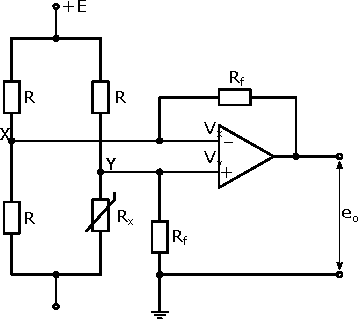
\includegraphics[width=0.7\linewidth]{fig/lec03/bridge_amp.pdf}
    \caption*{Bridge amplifier with resistive transducer}
\end{figure}
If \(a \ll 1\), then:
\begin{equation*}
e_o \approx \frac{E R_f}{R} a.
\end{equation*}

\textbf{Thus the circuit behaves linearly for small transducer changes.}
\end{columns}

\end{frame}

%=====================================================
\begin{frame}{Resistance Measurement}
\textbf{Goal}: Measure an unknown resistance \(R_X\) in situ, without disturbing its electrical environment.
\begin{columns}
\column{0.45\textwidth}
%\vspace{-25cm}
\begin{itemize}
    \item A known reference resistor \(R_s\) is fed from a reference source \(E_{ref}\).
    \item Current through \(R_s\) is forced through the unknown resistor \(R_X\).
    \item The op-amp holds point X at virtual earth (0 V), so all current must flow through \(R_X\).
\end{itemize}

\textbf{Key relationship:}
\begin{equation*}
e_o = \frac{E_{ref} R_X}{R_s}
\end{equation*}
Thus, the amplifier output voltage is \textbf{directly proportional} to the unknown resistance.
\column{0.55\textwidth}
\vspace{-0.5cm}
\begin{figure}
    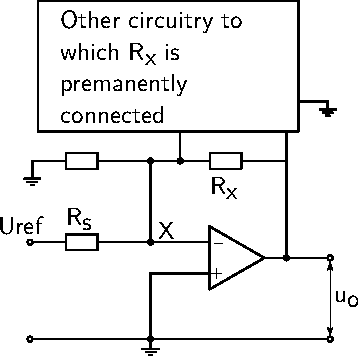
\includegraphics[width=0.5\linewidth]{fig/lec03/res_meas.pdf}
    \caption*{Resistance measurement circuit}
\end{figure}
\vspace{-0.5cm}
\textbf{Advantages}:
\begin{itemize}
\item Does not disturb existing circuitry connected to \(R_X\).
\item Virtual-earth node eliminates errors due to stray capacitances.
\end{itemize}

\end{columns}
\end{frame}

%=====================================================
\begin{frame}{Capacitance Measurement}
\textbf{Goal}: Measure small capacitances while eliminating errors due to stray capacitance to ground.
\begin{columns}
\column{0.6\textwidth}

Concept:
\begin{itemize}
    \item Connect unknown capacitor \(C_X\) to the inverting terminal.
    \item Op-amp maintains virtual earth at X \(\Rightarrow\) stray capacitances to ground carry negligible voltage.
    \item Known capacitor \(C_s\) is used in the feedback path.
\end{itemize}

\textbf{AC gain expression:}
\begin{equation*}
\frac{e_o}{e_i} = \frac{j \omega C_X R_f}{1 + j \omega C_s R_f}
\end{equation*}

Assuming:
\begin{equation*}
\omega \gg \frac{1}{2 \pi C_s R_f}
\end{equation*}

\column{0.4\textwidth}
\vspace{-0.5cm}
\begin{figure}
    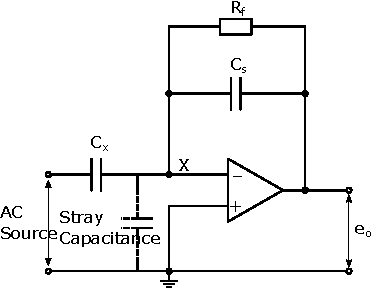
\includegraphics[width=0.6\linewidth]{fig/lec03/cap_measurement.pdf}
    \caption*{Capacitance measurement circuit}
\end{figure}

The output magnitude becomes approximately:
\begin{equation*}
C_X \approx \frac{e_o/e_i}{C_s}
\end{equation*}

\textbf{Important:} Choose \(C_s\) of the same order as \(C_X\) for accuracy.
\end{columns}
\end{frame}

%=====================================================
\begin{frame}{Air Speed Measurement}
\textbf{Principle}: Air flowing over a heated filament changes its resistance. This imbalance is sensed via a bridge and amplified.
\begin{columns}
\column{0.5\textwidth}

Process:
\begin{itemize}
    \item A platinum filament (positive temperature coefficient) is heated by a bias current.
    \item Cooling airflow reduces filament temperature, causing resistance \(R_f\) to decrease.
    \item The op-amp adjusts output voltage \(V_{out}\) to restore bridge balance.
    \item Thus: \textbf{output voltage is proportional to airflow speed}.
\end{itemize}


\column{0.5\textwidth}
\begin{figure}
    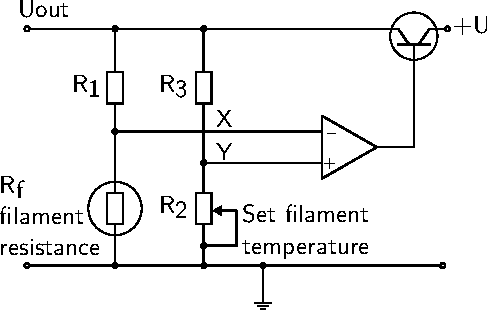
\includegraphics[width=0.8\linewidth]{fig/lec03/air_speed_measurement_2.pdf}
    \caption*{Air speed measurement using heated filament and bridge}
\end{figure}
\end{columns}
\end{frame}

%=====================================================
\begin{frame}{Air Speed Measurement}
\begin{columns}
\column{0.5\textwidth}
The bridge balance condition:
\begin{equation*}
R_f = \frac{R_1 R_2}{R_3}
\end{equation*}
\textbf{Advantages of constant-temperature anemometry}: 
\begin{itemize}
    \item Rapid response (no thermal lag).
    \item High sensitivity.
    \item Good linearity around the operating point.
\end{itemize}

\column{0.5\textwidth}
\begin{figure}
    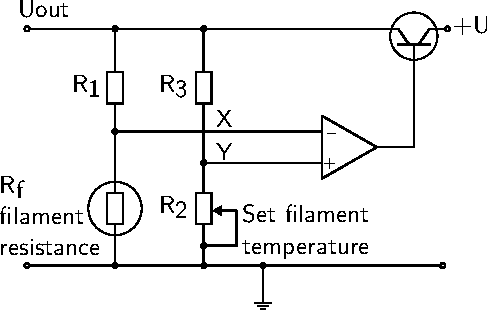
\includegraphics[width=0.8\linewidth]{fig/lec03/air_speed_measurement_2.pdf}
    \caption*{Air speed measurement using heated filament and bridge}
\end{figure}
\end{columns}

\end{frame}

\begin{frame}
{Additional Analogue Processing Circuits}

Beyond the circuits studied, many other analogue processing techniques exist:

\begin{itemize}
    \item \textbf{Capacitance multiplication}: simulate large capacitors using small ones + op-amp.
    \item \textbf{Arithmetic averaging amplifiers}: compute mean values.
    \item \textbf{Time-averaging filters}: perform low-pass smoothing.
    \item \textbf{Precision rectifiers and diode compensators}.
    \item \textbf{Ratiometric converters}: maintain accuracy against supply variations.
\end{itemize}
These can be explored further depending on course depth and student interest.
\end{frame}


\begin{frame}
    \begin{center}
            \Large{Noise in Measurement Systems}
    \end{center}
\end{frame}

% ==========================================================

\begin{frame}{What is Noise?}
    \begin{columns}
    \column{0.5\textwidth}
    \begin{block}{Definition}
    Noise is any \textbf{unwanted electrical signal} (voltage or current) that becomes intermixed with the wanted signal and degrades its readability.
    \end{block}

    \begin{itemize}
    \item In measurement systems, noise may originate from the sensor, wiring, environment, or electronics.
    \item If noise amplitude is comparable to or larger than the signal, \textbf{information can be lost}.
    \item Noise is typically \textbf{random} and described statistically (RMS, power spectral density).
    \end{itemize}

    \column{0.5\textwidth}
    \begin{figure}
    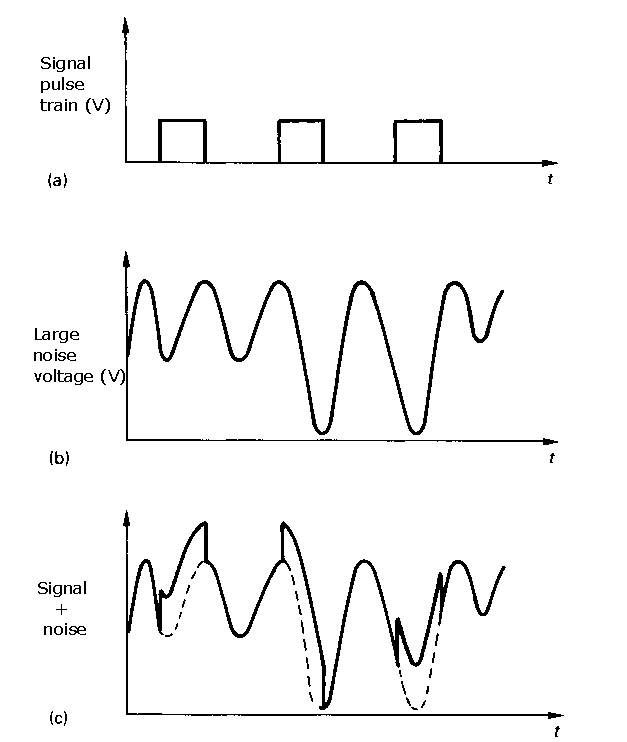
\includegraphics[width=0.75\linewidth]{fig/lec03/noise.pdf}
    \caption*{Signal corrupted by noise}
    \end{figure}

\end{columns}
\end{frame}

\begin{frame}{Internal vs External Noise}
    \begin{columns}[T,onlytextwidth]
    \column{0.45\textwidth}
    \begin{block}{Internal Noise}
    \begin{itemize}
    \item Generated \textbf{within} electronic components.
    \item Present even with zero input signal.
    \item Examples: thermal noise, shot noise, 1/f noise.
    \end{itemize}
    \end{block}

    \column{0.45\textwidth}
    \begin{block}{External Noise}
    \begin{itemize}
    \item Picked up \textbf{from surroundings}.
    \item Couples through stray capacitance, inductance, or radiation.
    \item Examples: mains interference, EMI from machines, lightning, radio transmitters.
    \end{itemize}
    \end{block}
\end{columns}

\vspace{0.2cm}
\textbf{Key idea:} External noise can often be reduced by design; internal noise sets the ultimate sensitivity limit.
\end{frame}

% ==========================================================


\begin{frame}{Signal-to-Noise Ratio (Linear Form)}
\begin{block}{Definition at a given frequency / bandwidth}
\begin{equation*}
\mathrm{SNR} = \frac{S}{N}
\end{equation*}
where
\begin{itemize}
  \item $S$ = wanted signal \textbf{power} in the band of interest \;[\unit{W}],
  \item $N$ = unwanted noise \textbf{power} in the same band \;[\unit{W}].
\end{itemize}
\end{block}

\begin{itemize}
  \item SNR is always defined for a \textbf{specified bandwidth} $B$.
  \item If the system bandwidth increases, noise power generally increases (often proportional to $B$).
\end{itemize}
\end{frame}

\begin{frame}{SNR in Decibels (dB)}
\begin{block}{Power ratio to decibels}
\begin{equation*}
\boxed{\mathrm{SNR}_{\mathrm{dB}} = 10\log_{10}\!\left(\frac{S}{N}\right) \unit{dB}}
\end{equation*}
\end{block}

\textbf{Voltage or current ratios:}
\begin{itemize}
  \item When signal and noise are measured as \textbf{RMS voltages} across the same resistance $R$:
  \begin{equation*}
  \frac{S}{N} = \left(\frac{V_{S,\mathrm{rms}}}{V_{N,\mathrm{rms}}}\right)^2
  \quad \Rightarrow \quad
  \mathrm{SNR}_{\mathrm{dB}} = 20\log_{10}\!\left(\frac{V_{S,\mathrm{rms}}}{V_{N,\mathrm{rms}}}\right)
  \end{equation*}
  \item Similarly for currents: \;$\mathrm{SNR}_{\mathrm{dB}} = 20\log_{10}(I_{S,\mathrm{rms}}/I_{N,\mathrm{rms}})$.
\end{itemize}

\textbf{Note:} Amplifier gain does \emph{not} improve input SNR; it amplifies signal and noise alike, and adds its own noise.
\end{frame}

\begin{frame}{Example of SNR Calculation}
Suppose an amplifier input has:
\begin{itemize}
  \item wanted signal power: $S = 3\unit{mW}=3\times10^{-3}\unit{W}$,
  \item noise power: $N = 30\unit{\mu W}=30\times10^{-6}\unit{W}$.
\end{itemize}

\begin{align*}
\mathrm{SNR} &= \frac{S}{N} = \frac{3\times10^{-3}}{30\times10^{-6}} = 100 \\
\Rightarrow \mathrm{SNR}_{\mathrm{dB}} &= 10\log_{10}(100)=10\times 2 = 20\unit{dB}
\end{align*}

\begin{itemize}
  \item $20\unit{dB}$ may be acceptable for voice links, but high-quality audio typically needs $>60\unit{dB}$.
\end{itemize}
\end{frame}

% ==========================================================

\begin{frame}{Overview of External Noise Sources}
\begin{itemize}
  \item External noise includes all unwanted signals \textbf{picked up} from the environment.
  \item Coupling paths:
  \begin{itemize}
    \item \textbf{Capacitive coupling} via stray capacitances $C_s$.
    \item \textbf{Inductive coupling} via changing magnetic fields and loop areas.
    \item \textbf{Radiated EMI} through space at RF.
    \item \textbf{Conducted interference} through shared supplies/grounds.
  \end{itemize}
  \item We focus on three representative groups:
  \begin{enumerate}
    \item mains interference (50/60\unit{Hz}),
    \item other man-made interference,
    \item natural noise sources.
  \end{enumerate}
\end{itemize}
\end{frame}


\begin{frame}{Mains Interference (50/60 Hz Pick-up)}
    \begin{columns}
    \column{0.5\textwidth}

\begin{itemize}
  \item A common external noise is coupling from the mains power line.
  \item Stray capacitances $C_s$ between power lines and signal wiring inject a small 50\unit{Hz} component.
  \item Not only the fundamental (50\unit{Hz}) but also harmonics (100, 150\unit{Hz}, \ldots) may appear.
\end{itemize}
\textbf{Mitigation preview:}
\begin{itemize}
  \item increase physical separation of power and signal wiring,
  \item reduce loop area,
  \item use shielding and single-point grounding (next section).
\end{itemize}

    \column{0.5\textwidth}
\begin{figure}
    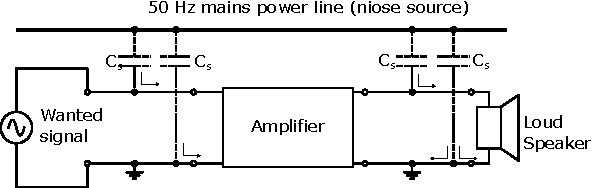
\includegraphics[width=0.8\linewidth]{fig/lec03/noise2.pdf}
    \caption*{Capacitive coupling of mains interference}
\end{figure}

\end{columns}
\end{frame}

\begin{frame}{Conductive Sheath / Shield Against Mains Pick-up}
    \begin{columns}
    \column{0.5\textwidth}
    \begin{itemize}
  \item Enclosing sensitive wiring/equipment in a conductive sheath tied to a \textbf{single earth point} can block capacitive coupling.
  \item The sheath provides a low-impedance return for displacement currents induced via $C_s$.
\end{itemize}


\begin{block}{Key takeaway}
Good shielding requires a clear reference node; multiple earth points may create earth-loop noise.
\end{block}
    \column{0.5\textwidth}
    \begin{figure}
    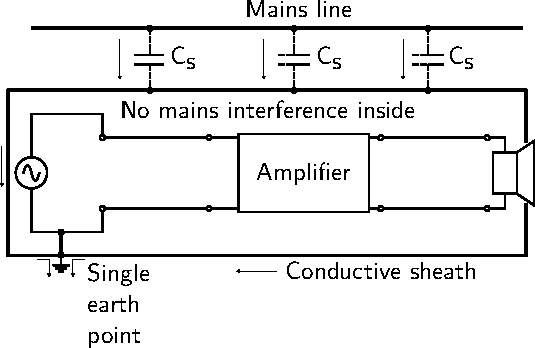
\includegraphics[width=0.8\linewidth]{fig/lec03/noise3.pdf}
    \caption*{Shielded cable to reduce mains pick-up}
    \end{figure}
    \end{columns}

\end{frame}


\begin{frame}{Other Man-made Noise Sources}
\begin{itemize}
  \item Generated by nearby electrical/electronic equipment.
  \item Examples:
  \begin{itemize}
    \item sparking commutators and brushes in DC/universal motors,
    \item fluorescent lamps and switching power supplies,
    \item switchgear producing rapid $di/dt$ and $dv/dt$ transients,
    \item radio/telemetry equipment.
  \end{itemize}
  \item Often broadband and impulsive; can fall inside measurement band.
\end{itemize}

\vspace{0.2cm}
\textbf{Three important mechanisms:}
\begin{enumerate}
  \item adjacent channel interference,
  \item cross-talk between cables,
  \item intermodulation products in non-linear devices.
\end{enumerate}
\end{frame}

\begin{frame}{Other Man-made Noise Sources}
    \begin{columns}
    \column{0.5\textwidth}

    \textbf{Adjacent Channel Interference}
\begin{itemize}
  \item In radio/data systems, channels operate at carrier frequencies $f_1, f_2, \ldots$.
  \item A strong interferer on a nearby channel may leak into the wanted channel if filtering is insufficient.
  \item Mitigation:
  \begin{itemize}
    \item better frequency-selective front-end filtering,
    \item adequate geographical/physical separation,
    \item proper antenna orientation/polarization.
  \end{itemize}
\end{itemize}

    \column{0.5\textwidth}
\textbf{Cross-talk Between Cables}
\begin{itemize}
  \item When two or more cables run close together, changing currents create magnetic fields that induce voltages in adjacent conductors.
  \item Electrostatic coupling between conductors adds capacitive cross-talk.
  \item Mitigation:
  \begin{itemize}
    \item route sensitive and noisy cables separately,
    \item use twisted pairs and screened (shielded) cables,
    \item minimize parallel run length.
  \end{itemize}
\end{itemize}
    \end{columns}
\end{frame}


\begin{frame}{Intermodulation Noise}
\begin{itemize}
  \item Two signals at $f_1$ and $f_2$ passing through a non-linear device produce new frequencies:
  \begin{equation*}
  f_1,\; f_2,\; f_1+f_2,\; |f_1-f_2|,\; 2f_1,\; 2f_2,\; \dots
  \end{equation*}
  \item Some products may lie within the measurement band and degrade SNR.
  \item Mitigation:
  \begin{itemize}
    \item avoid device saturation/non-linear regions,
    \item band-limit before non-linear stages,
    \item maintain adequate headroom.
  \end{itemize}
\end{itemize}
\end{frame}


\begin{frame}{Natural Noise Sources}
\begin{itemize}
  \item Predominantly affects radio-frequency and long-distance sensing.
  \item Two common types:
  \begin{enumerate}
    \item \textbf{Atmospheric / static noise} from lightning and electric storms.
    \item \textbf{Galactic / cosmic noise} from stars and solar activity.
  \end{enumerate}
\end{itemize}

\begin{block}{Frequency ranges}
\begin{itemize}
  \item Atmospheric noise is significant up to about $25\unit{MHz}$.
  \item Cosmic noise dominates beyond $\sim 1\unit{GHz}$.
\end{itemize}
\end{block}
\end{frame}

% ==========================================================

\begin{frame}{Suppression Strategies: Big Picture}
\begin{itemize}
  \item External noise suppression depends on:
  \begin{itemize}
    \item frequency content of the interference,
    \item power level of the noise source,
    \item sensitivity/bandwidth of the measurement chain.
  \end{itemize}
  \item Three practical levers:
  \begin{enumerate}
    \item \textbf{Shielding},
    \item \textbf{Good circuit layout},
    \item \textbf{Eliminating earth loops}.
  \end{enumerate}
\end{itemize}
\end{frame}


\begin{frame}{Suppression Strategies}
    \begin{columns}
    \column{0.45\textwidth}

\begin{itemize}
  \item \textbf{Electrostatic (capacitive) shielding}:
  \begin{itemize}
    \item Use a conductive enclosure tied to earth.
    \item Provides low-impedance path for displacement currents.
  \end{itemize}
  \item \textbf{Magnetic shielding at low frequency}:
  \begin{itemize}
    \item Use high-permeability materials (e.g., mu-metal- nickel-iron soft alloy).
    \item Offers a low-reluctance path to divert interfering flux.
  \end{itemize}
  \item \textbf{RF shielding (skin effect)}:
  \begin{itemize}
    \item A low-resistance metal shield (Al, Cu, brass).
    \item Incident RF flux induces eddy currents; their opposing field cancels penetration.
  \end{itemize}
\end{itemize}

    \column{0.45\textwidth}
    \textbf{Practical Shielding Techniques}
    \begin{itemize}
    \item Braided shields or coaxial cables for signal lines.
    \item Mesh shields can reduce electrostatic noise while staying lightweight.
    \item Always maintain \textbf{continuous shield connection} to reference (avoid floating ends unless designed as such).
    \end{itemize}

    \begin{block}{Pitfall}
    Multiple shield earth points can create circulating currents (earth loops), re-introducing noise.
    \end{block}
\end{columns}
\end{frame}


\begin{frame}{Good Circuit Layout}
\begin{itemize}
  \item Keep mains / high-current tracks \textbf{far from} low-level signal paths.
  \item Avoid shared routing of power and signal through the same trunking or conduit.
  \item Minimize loop areas in sensitive circuits to reduce inductive pick-up.
  \item Use star-ground or single-point reference where possible.
\end{itemize}

\begin{block}{Rule of thumb}
Treat layout as part of the circuit: parasitic $C_s$ and mutual inductance are layout-controlled components.
\end{block}
\end{frame}


\begin{frame}{Earth Loops (Ground Loops) Concept and Mitigation}
    \begin{columns}
    \column{0.6\textwidth}

\begin{itemize}
  \item An earth loop occurs when a system has \textbf{more than one earth bond}.
  \item Different earth potentials ($e_A \neq e_B$) drive a loop current that couples into the signal path.
  \item The loop acts like an aerial, picking up magnetic/electric interference.
\end{itemize}
\begin{itemize}
  \item Use a \textbf{single-point earth} (star grounding).
  \item Avoid ground connections through multiple equipment chassis.
  \item If unavoidable, break loops with:
  \begin{itemize}
    \item differential inputs / instrumentation amplifiers,
    \item isolation (transformer, opto-isolator),
    \item careful cable shielding strategy.
  \end{itemize}
\end{itemize}

    \column{0.4\textwidth}
\begin{figure}
    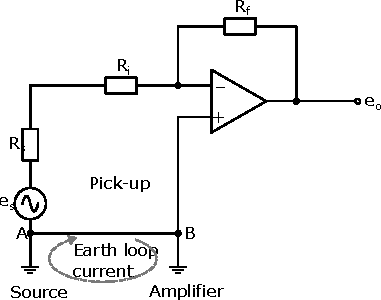
\includegraphics[width=0.9\linewidth]{fig/lec03/noise4.pdf}
    \caption*{Example of an earth loop}
\end{figure}
    \end{columns}
\end{frame}



% ==========================================================

\begin{frame}{Why Internal Noise Matters}
\begin{itemize}
  \item Even with perfect shielding, every resistor, semiconductor, and amplifier generates noise.
  \item Internal noise sets the ultimate \textbf{minimum detectable signal}.
  \item We focus on three core types:
  \begin{enumerate}
    \item thermal (Johnson) noise,
    \item shot noise,
    \item flicker (1/f) noise.
  \end{enumerate}
\end{itemize}
\end{frame}


\begin{frame}{Thermal (Johnson) Noise in Resistors}
\begin{itemize}
  \item Caused by random thermal motion of charge carriers.
  \item Produces a noise voltage with zero mean but non-zero RMS.
  \item Spread uniformly over frequency \(\rightarrow\) \textbf{white noise}.
\end{itemize}

\begin{block}{RMS noise voltage over bandwidth $B$}
\begin{equation*}
\boxed{E_n = \sqrt{k_{\mathrm{B}} T B R}}
\end{equation*}
where
\begin{itemize}
  \item $k_{\mathrm{B}}$ = Boltzmann constant $\approx 1.38\times10^{-23}\unit{J/K}$,
  \item $T$ = absolute temperature,
  \item $B$ = bandwidth,
  \item $R$ = resistance.
\end{itemize}
\end{block}

\textbf{Implication:} doubling $B$ increases $E_n$ by $\sqrt{2}$ and increases noise \emph{power} by 2.
\end{frame}

\begin{frame}{Thermal Noise: Key Design Insights}
\begin{itemize}
  \item Noise scales with \textbf{temperature}: cooling reduces $E_n$.
  \item Noise scales with \textbf{resistance}: larger $R$ gives larger noise voltage.
  \item Noise scales with \textbf{bandwidth}: keep $B$ only as wide as needed.
  \item Equivalent noise power in $R$:
  \begin{equation*}
  P_n = \frac{E_n^2}{R} = 4k_{\mathrm{B}} T B \;\unit{W}
  \end{equation*}
  (note independence from $R$ for a matched load).
\end{itemize}
\end{frame}


\begin{frame}{Shot Noise in Semiconductors}
\begin{itemize}
  \item Due to discrete nature or random variations in the flow of charge / carriers crossing junctions.
  \item Dominant when DC current passes through a diode/transistor junction.
  \item Also noise power uniform across frequency spectrum -- white over frequency (within typical bands).
\end{itemize}

\begin{block}{RMS shot-noise current}
\begin{equation*}
\boxed{i_n = \sqrt{2 e I B}\;\unit{A}}
\end{equation*}
where
\begin{itemize}
  \item $e$ = electronic charge $\approx 1.60\times10^{-19}\unit{C}$,
  \item $I$ = DC junction current \;[\unit{A}],
  \item $B$ = bandwidth \;[\unit{Hz}].
\end{itemize}
\end{block}

\textbf{Takeaway:} higher DC current $I$ increases shot noise proportionally to $\sqrt{I}$.
\end{frame}


\begin{frame}{Flicker Noise (1/f or Pink Noise)}
\begin{itemize}
  \item Arises from random trapping/recombination in semiconductors.
  \item Magnitude increases as frequency decreases.
  \item Often significant below about $10\unit{Hz}$.
\end{itemize}

\begin{block}{Spectral form (qualitative)}
Noise power spectral density typically follows
\begin{equation*}
S_{1/f}(f) \propto \frac{1}{f^{\alpha}},\quad \alpha\approx 1.
\end{equation*}
\end{block}

\textbf{Practical meaning:} low-frequency measurements (slow sensors, DC offsets) are most affected.
\end{frame}

\begin{frame}{Partition Noise}
\begin{itemize}
  \item Occurs in transistors because emitter current divides randomly between base and collector.
  \item Can be viewed as an additional internal current-noise source.
  \item Usually smaller than thermal/shot noise but relevant in precision low-level circuits.
\end{itemize}

\begin{itemize}
  \item Additional noise-reduction and signal-conditioning methods exist:
  \begin{itemize}
    \item capacitance multiplication, arithmetic/time averaging,
    \item chopper stabilization, modulation/demodulation,
    \item digital filtering and oversampling.
  \end{itemize}
  \item We will explore these in advanced sessions or projects.
\end{itemize}
\end{frame}

% ==========================================================

\begin{frame}{Summary}
\begin{itemize}
  \item Noise is the unavoidable unwanted part of any measurement.
  \item \textbf{SNR} quantifies quality; in dB:
  $\mathrm{SNR}_{\mathrm{dB}}=10\log_{10}(S/N)$.
  \item External noise can be reduced through shielding, layout, and ground-loop elimination.
  \item Internal noise types:
  \begin{itemize}
    \item Thermal: $E_n=\sqrt{4k_{\mathrm{B}} T B R}$.
    \item Shot: $i_n=\sqrt{2eIB}$.
    \item Flicker: $S_{1/f}(f)\propto 1/f$.
  \end{itemize}
  \item Design for low noise means: minimize bandwidth, resistance where possible, and avoid non-linear operation.
\end{itemize}
\end{frame}


